\subsection{Embedding statico: GloVe}
\textbf{GlobalVectors} (GloVe) è un modello assai noto che apprende i vettori o le parole dalle informazioni di co-occorrenza, ovvero la frequenza con cui compaiono insieme in grandi corpora di testo. GloVe è basato sul conteggio. In linea generale i modelli basati sul conteggio apprendono i vettori, operando una riduzione della dimensionalità sulla matrice di conteggio delle co-occorrenze.

Per prima cosa, si costruisce una grande \textbf{matrice di co-occorrenza} (parole x colonne), che contiene le informazioni sulla frequenza con cui ogni parola viene usata in un contesto. Il numero di contesti deve essere grande, poiché è essenzialmente di dimensioni combinatorie.

In seguito, tale matrice viene riscritta in forma algebrica e fattorizzata per ottenerne una dimensionalmente più piccola. Il risultato di questa operazione è una rappresentazione vettoriale per ogni parola.

L’addestramento può poi essere eseguito in due modi diversi: utilizzando il contesto per predire una parola target (utilizzando metodi noti come il BoW\textsuperscript{\cite{bow_article}} o il CBoW\textsuperscript{\cite{mikolov2013efficient}}) oppure usando una parola per predirre il contesto target (Skip-Gram\textsuperscript{\cite{skipgram}}).
% Precisamente, l'algoritmo GloVe consiste nei seguenti passi:
% \begin{enumerate}
%     \item Raccogliamo le statistiche di co-occorrenza delle parole in una forma di matrice di co-occorrenza di parole \(X\). Ogni elemento \(X_i_j\) di tale matrice rappresenta quanto spesso la parola \(i\) appare nel contesto della parola \(j\). Di solito scansioniamo il nostro corpus nel seguente modo: per ogni termine cerchiamo termini contestuali entro una certa area definita da una costante chiamata \(dimensione_finestra\) prima del termine e una \(dimensione_finestra\) dopo il termine. 
%     \clearpage
%     \begin{figure}[hbt!]
%         \centering
%         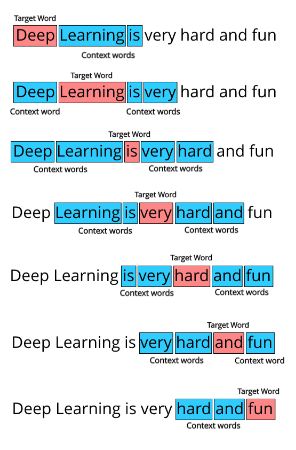
\includegraphics[width=0.5\textwidth]{img/context_window.png}
%         \caption{Context Window}
%         \label{fig:context_window}
%     \end{figure} \\
%     Inoltre diamo meno peso alle parole più lontane, di solito usando questa formula:
%     \begin{center}
%         \(decay=1/offset\)
%     \end{center}
    
%     \item Definiamo i vincoli per ogni coppia di parole:
%     \begin{center}
%         \(w^T_i w_j + b_i + b_j = log(X_i_j)\)
%     \end{center}
%     dove \(w_i\) è il vettore per la parola principale, \(w_j\) è il vettore per la \textit{context word}, \(b_j, b_j\) sono bias scalari rispettivamente per la parola principale e di contesto
    
%     \item Definiamo una funzione di costo:
%     \begin{center}
%         \[J = \sum_{i=1}^{V} \sum_{j=1}^{V} f(X_i_j)(w^T_i w_j + b_i + b_j - log(X_i_j))^2\]
%     \end{center}
%     Qui \(f\) è una funzione di ponderazione che ci aiuta a prevenire l'apprendimento solo da coppie di parole estremamente comuni. Gli autori di GloVe hanno scelto la seguente funzione:
%     \begin{center}
%         \[ f(X_i_j) = 
%           \begin{cases} 
%                 (\frac{X_i_j}{X_m_a_x})^\alpha & if X_i_j < X_m_a_x \\
%                 1 & otherwise
%             \end{cases}
%         \]
%     \end{center}
% \end{enumerate}